\subsection{Total Score and Sensitivity}

From Section \ref{sec:scoring_outline}, it can be concluded that in case all mission requirements are met, the only opportunity for the score improvement lies in Written Report Score and RAC. Thus, a sensitivity analysis has been performed to asses the impact of different configurations on RAC.\\

Three different configurations have been analysed as the most viable ones: 
\begin{itemize}
    \item $\text{N}_{\text{comp}}$ = 1, 1 laps in Mission 2
    \item $\text{N}_{\text{comp}}$ = 2, 2 laps in Mission 2
    \item $\text{N}_{\text{comp}}$ = 2, 1 lap in Mission 2
\end{itemize}

3 components option was also considered for different numbers of laps in Mission 2, however it would always produce higher RAC, since with $\text{N}_{\text{comp}} = 3$,  $\text{EW}_{1} \times \text{Wt}_{\textrm{Battery 1}} \times \text{N}_{\text{comp}}$ outweighs any benefit obtained by reducing $\text{EW}_{2} \times \text{Wt}_{\textrm{Battery 2}}$.\\

First analysed 1 flight 1 component vs 2 flight 2 components!\\


The analysis was primarily based on the ratio of $m_{{ac}}$ to $m_{payload}$ and $m_{{ac}}$ to $m_{battery}$. Those ratios were defined separately for 3 different configurations and were determined to be the main variables defining the RAC. The ratios were initially taken based on team's previous experience as well as past competition reports. The initial ratios can be found in Table \ref{fig:sens_constants}. \\

\begin{figure}[!h]
    \centering
    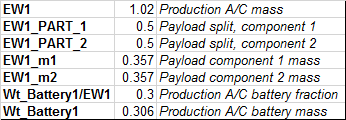
\includegraphics{sens_constants}
    \caption{Experienced based initial conditions \_PLACEHOLDER }
    \label{fig:sens_constants}
\end{figure}

Part below is analysis of 1 flight N=2 vs 2 flight N=2.\\

The aircraft carrying 2 components at the same time would have to carry a higher payload than the aircraft making 2 flights and carrying 1 component at a time. If the design is well optimised, it would mean that the former would require a heavier structure than the latter. Also, carrying more structural mass and having to take off with a higher payload, it would require more power for takeoff, and hence the propulsion mass would be higher as well. On the other hand, splitting the Production aircraft with chosen configuration to two components means that in terms of external dimensions, practically identical fuselage is required to carry either 1 component or 2 components. This means that 1 lap 2 components Manufacturing Aircraft configuration is likely to be more volume efficient, and thus it should be possible to achieve a better payload ratio. For that reason, it was always assumed that 2 components, 1 lap option Manufacturing Support Aircraft will have a lower mass of aircraft to mass of payload ratio.\\

Since Mission 1 requires the Manufacturing Aircraft to be able to fly 3 laps, it was first assumed that meeting this requirement would automatically allow flying 2 laps tp carry 2 components in Mission 2. The later concern was, however, that NiMH cells are known to produce less power after some discharge, and there might be a requirement to have a higher capacity battery to be able to produce the required power for the second takeoff in $\text{N}_{\text{comp}} = 2$, 2 laps case. For that purpose a number of the most likely ratios of $\text{EW1} / m_{payload}$ were identified. Then the RAC was calculated for a baseline case for both configuration, assuming the battery mass would be $30\%$ of the EW2. From that baseline, the battery mass fraction for 2 components, 2 flights option was changed to match the RAC of 2 components, 1 flight. This provides the headroom available for battery mass increase, as can be seen in Table \ref{fig:sens_config}.

\begin{figure}[!h]
    \centering
    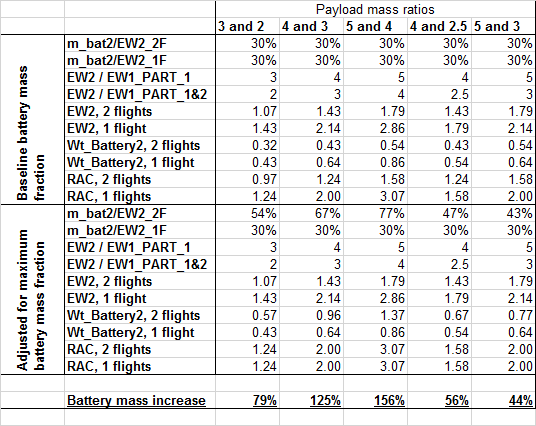
\includegraphics{sens_config}
    \caption{Number of flights for $\text{N}_{\text{comp}} = 2$ battery sensitivity analysis \_PLACEHOLDER }
    \label{fig:sens_config}
\end{figure}



As can be seen, there is plenty of battery mass penalty headroom for even the most conservative payload ratios, which implies that 2 components, 2 laps option will allow getting the highest RAC and thus the highest score possible.

how to determine number of components and flights\\



briefly intro 3 comnp 3 flights\\


%%%%%%%%%%%%%%%%%%%%%%%%%%%%%%%%%%%%%%%%%%%%%%%%%%%%%%%%%%%%%%%%%%%%%%%%%%%%%%%%%%%%%%
%%%%%%%%%%%%%%%%%%%%%%%%%  		CONFIGURATION SELECTION		 %%%%%%%%%%%%%%%%%%%%%%%%%
%%%%%%%%%%%%%%%%%%%%%%%%%%%%%%%%%%%%%%%%%%%%%%%%%%%%%%%%%%%%%%%%%%%%%%%%%%%%%%%%%%%%%%